\documentclass[11pt]{beamer}
%\usetheme[faculty=fi,nofonts]{fibeamer}
\usetheme[
  workplace=fi,
]{MU}

\usepackage[utf8]{inputenc}
\usepackage[czech]{babel}
\usepackage[T1]{fontenc}
\usepackage{amsmath}
\usepackage{amsfonts}
\usepackage{amssymb}
\usepackage{amsthm}
\usepackage{graphicx}
\usepackage{listings}
\usepackage[margin=1.5cm]{caption}
\usepackage{float}

\author{Jan Tušil}
\title{Angelic Verification}
\subtitle{Precise Verification Modulo Unknowns}
%\setbeamercovered{transparent} 
%\setbeamertemplate{navigation symbols}{} 
%\logo{} 
%\institute{} 
%\date{2018-03-23} 
%\date{2018-03-23} 
%\subject{} 

\newtheorem{dfn}{Definice}

%\floatstyle{boxed} 
%\restylefloat{figure}

%\floatstyle{boxed}
%\newfloat{program}{thp}{lop}
%\floatname{program}{Program}

\lstset{
numbers=left, 
numberstyle=\small, 
numbersep=8pt, 
frame = single, 
%language=Pascal, 
framexleftmargin=15pt
}

\begin{document}

% Ahoj,
% dneska se budeme věnovat článku zvaném "Angelic Verification: Precise
% Verification Modulo Unknowns", který vyšel na CAVu v roce 2015.
% Myšlenky z tohoto článku byly implementovány v nástroji
% AngelicVerifier, a autoři (z Microsoftu) tvrdí, že je tento nástroj může soutěžit
% s nástroji SDV a PREfix, ovšem s výrazně nižšími nároky na práci uživatele.
\begin{frame}
\titlepage
\end{frame}

% Obsah: motivace, maso, porovnání.
\begin{frame}
\tableofcontents
\end{frame}

% Otevřené a uzavřené programy, plané poplachy
\section{Motivace}

% Začněme příkladem.

% Řekněme, že máme nástroj, kterému předhodíme program a on nám řekne,
% jestli existuje běh tohoto programu z nějakého iniciálního stavu
\begin{frame}[fragile]{Uzavřený program}


\end{frame}

% Zabýváme se hledáním běhových chyb či prokazováním jejich absence.
% Chyby jsou modelovány selhanými asserty.

% Hmm... ta otevřenost může způsobit plané poplachy,
% které jsou plané v tom smyslu, že předpokládají nějaké použití programu,
% které v reálu nenastane - třeba proto, že ten program pro něj není urrčený.


% Uvažme například tento program v jazyce Boogie,
% který vznikl zakletím nějakého programu z jazyka C.
% Přičemž ukazatele jsou zde modelovány jako čísla, která jsou následně
% použitá pro indexování pole m.

% Za vstupní bod považujme proceduru Foo.
% Hmm... nebo klidne vsechny

% Jaké jsou zde zdroje neznámých, neomezených hodnot?
% (Parametr z, procedury Lib1, Lib2).
% Které z těchto assertů mohou selhat?
% Ve vší obecnosti, pokud o neznámých hodnotách nic nepředpokládáme,
% mohou selhat všechny. Přesto, když programátor dostane
% od nástroje pět varování, nebude z nich úplně nadšený
% - on přece ví, že funkce Lib2 nevrací NULL.
% Bylo by fajn tahle varování nějak seřadit,
% třeba podle toho, jak jsou užitečná.

% Chya určitě při volání baz. Nejspíš ano v bar - nekonzistence.
% Asi ne pro FooBar. Je celkem rozumné předpokládat, že daná knihovní funkce nevrací NULL.
\begin{frame}{Otevřený program - plané poplachy}
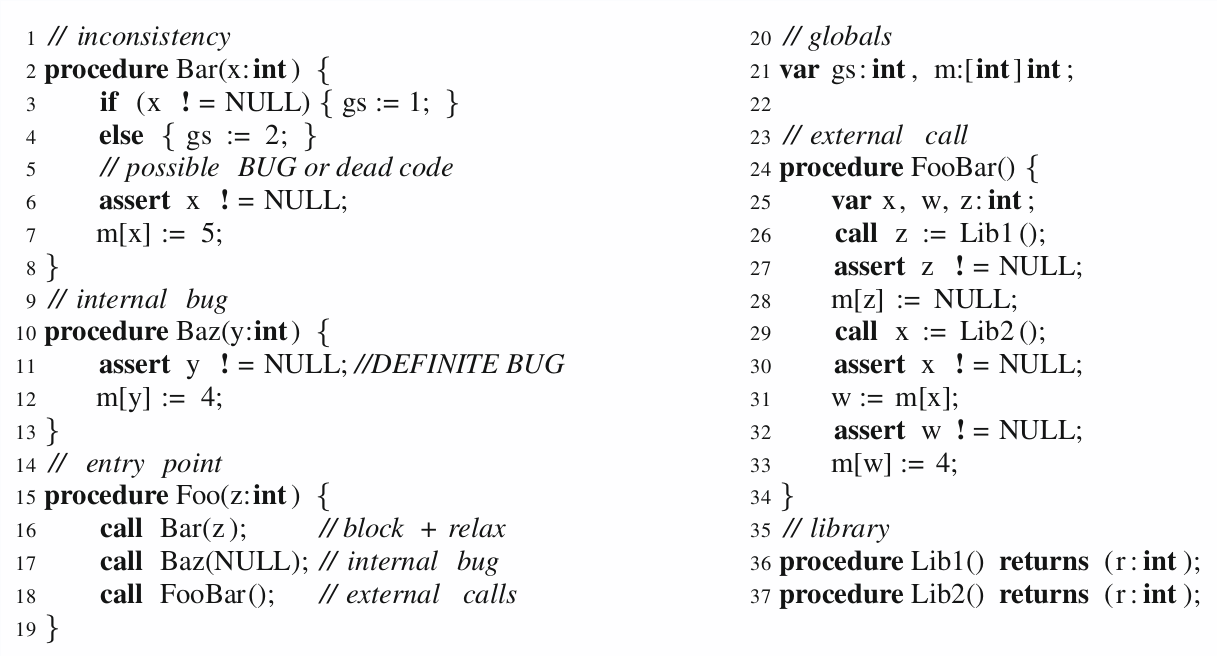
\includegraphics[width=1.0\linewidth]{img/exampleProgram.png}
\end{frame}

\begin{frame}[fragile]{Některé stopy programu}
\begin{lstlisting}
push; // call bar
gs := 2;
assert x != null;
fail;
\end{lstlisting}
\end{frame}

\begin{frame}[fragile]
\begin{lstlisting}
int gs;
void bar(int *x) {
  if (x != nullptr) gs = 1;
  else gs = 2;
  *x = 5;
}

void baz(int *y) {
  *y = 4;
}

void foo(int *z) {
  bar(z);
  baz(nullptr);
}

int ** Lib1();
int ** Lib2();
void FooBar() {
  *Lib1() = NULL;
  **Lib2() = 4;
}
\end{lstlisting}
\end{frame}


\begin{frame}{Cíl}
\begin{itemize}
\item cíl: prioritizace důležitějších alarmů
\item  metoda: angelická verifikace (i.e. abduktivní inference)
\end{itemize}

\begin{dfn}[Problém angelické verifikace]
Pro daný assert, existuje rozumná specifikace nad neznámými hodnotami taková,
že daný assert platí?
\end{dfn}

\end{frame}

\section{Detaily}


\begin{frame}{Přijatelná specifikace}
Chceme, aby přijatelná specifikace byla:
\begin{itemize}
\item stručná
\item shovívavá
\end{itemize}
\end{frame}

\begin{frame}{Shovívavá vstupní podmínka}
\begin{dfn}[Shovívavá vstupní podmínka]
Formule $\phi$ je shovívavá vstupní podmínka programu $P_{A, \hat{A}}$,
značíme $Permissive\left( P_{A, \hat{A}}, \Phi \right)$,
pokud pro každý andělský assert $s \in \hat{A} $ platí:
pokud $\phi \vDash P_{\emptyset, \{ s \} }$, pak  $ \texttt{true} \vDash P_{\emptyset, \{ s \} } $.
\end{dfn}

\pause Jak to říci jinak?

\pause Jak vypadají shovívavé vstupní podmínky programu, který obsahuje andělský
\begin{itemize}
\pause \item \lstinline|assert false| na začátku programu?
\pause \item \lstinline|assert false| na konci každého bloku?
\pause \item \lstinline|assert x != v| někde?
\end{itemize}

\end{frame}

\begin{frame}{Andělská korektnost}
\begin{dfn}
Mějme program P obsahující sadu běžných assertů $A$
a sadu andělských assertů $\hat{A}$, spolu se slovníkem formulí \texttt{Vocab}.
Říkáme, že P je andělsky korektní za předpokladu $( \texttt{Vocab}, \hat{A} )$,
pokud existuje formule $\phi \in \textsf{Vocab}$, která je shovívavou vstupní podmínkou programu P,
a přitom $\phi \vDash P_{A, \emptyset}$. 
\end{dfn}
\end{frame}


% Předpokládejme, že máme funkci Verify, které můžeme předhodit
% program a vstupní podmínku. Tato funkce rozhodne,
% každý z běhů, jejichž iniciální stav splňuje vstupní podmínku,
% naplní asserty. Pokud ne, vrátí takovýto běh.

% Algoritmus pro angelickou verifikaci funguje tak,
% že začíná s prázdnou specifikací (tj. true), 
% a postupně ji zjemňuje tak dlouho,
% dokud v programu stále existuje chybový běh.
% Z tohoto chybového běhu se vyextrahuje formule,
% která tento běh blokuje, a přidá se do specifikace.

% Může se ale stát, že takovou formuli nebudeme schopni najít,
% nebo bude vzniklá specifikace příliš tvrdá (nebude shovívavá)
% - například nebude vůbec splnitelná. V takovém případě algoritmus novou formuli nepoužije
% a odebere selhávající assert z množiny assertů, které se snaží dokázat.
\begin{frame}{AngelicVerifier}
\begin{columns}

\begin{column}{0.5\textwidth}
\pause 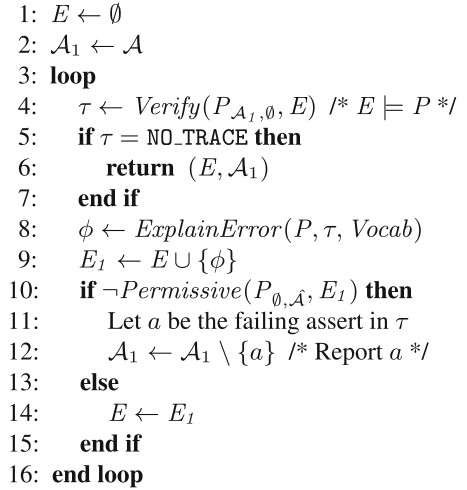
\includegraphics[width=0.9\linewidth]{img/angelicVerifyShort.png}
\end{column}

\begin{column}{0.5\textwidth}
\begin{itemize}
\pause \item Vstupy: program $P$ s obyčejnými asserty $A$ a andělskými asserty $\hat{A}$.
\pause \item Výstupy: shovívavá specifikace $E$ a množina platících obyčejných assertů $A_1 \subseteq A$.
\pause \item $\phi$ - formule blokující chybový běh $\tau$
\end{itemize}
\end{column}

\end{columns}
\end{frame}

\begin{frame}{ExplainError}
\begin{columns}

\begin{column}{0.5\textwidth}
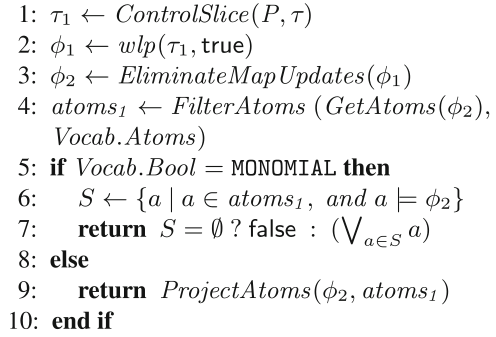
\includegraphics[width=0.9\linewidth]{img/explainErrorShort.png}
\end{column}

\begin{column}{0.5\textwidth}
Explanation
\end{column}

\end{columns}
\end{frame}

\begin{frame}[fragile]{Příklad}
\begin{columns}

\begin{column}{0.5\textwidth}<1->
%\begin{figure}
\frame{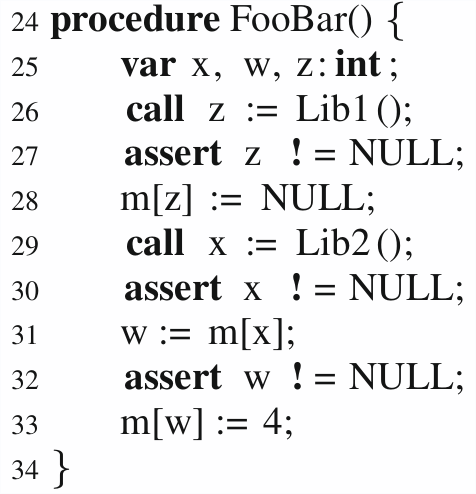
\includegraphics[width=0.9\textwidth]{img/fooBar.png}}
%\caption{Stopa se selhávajícím assertem.}
%\end{figure}
\end{column}

\begin{column}{0.5\textwidth}<2>
Stopa $\tau$:
\begin{lstlisting}
z := x_1;
m[z] := NULL;
x := x_2;
w := m[x];
assert w != NULL;
\end{lstlisting}

\begin{itemize}
%\item stopa = program bez řídících struktur
\item volání knihovních procedur nahrazena novými proměnnými
\end{itemize}

% $$wlp(\tau, true) = \textsc{read}(write(m, x_1, NULL), x_2) $$

\end{column}

\end{columns}
\end{frame}


% Klasický WP kalkulus s tím, že čtení a zápis
% do polí modelujeme pomocí funkcí read a write.
% Formule nad jazykem polí, arithmetiky, a rovností.
% Zkusíme si to na tabuli sami spočítat
\begin{frame}[fragile]{Příklad}
%\begin{columns}

%\begin{column}{0.5\textwidth}<1>
Stopa $\tau$:
\begin{lstlisting}
z := x_1;
m[z] := NULL;
x := x_2;
w := m[x];
assert w != NULL;
\end{lstlisting}

\pause

$wlp(\tau, true)$:
\begin{lstlisting}
read(write(m, x_1, NULL), x_2)
\end{lstlisting}

\pause 

EliminateMapUpdates:
\begin{lstlisting}
x_2 == x_1 ? NULL : read(m, x_1)
\end{lstlisting}

%\end{column}
%\end{columns}
\end{frame}


\end{document}